%%
%% This is file `./samples/longsample.tex',
%% generated with the docstrip utility.
%%
%% The original source files were:
%%
%% apa7.dtx  (with options: `longsample')
%% ----------------------------------------------------------------------
%% 
%% apa7 - A LaTeX class for formatting documents in compliance with the
%% American Psychological Association's Publication Manual, 7th edition
%% 
%% Copyright (C) 2021 by Daniel A. Weiss <daniel.weiss.led at gmail.com>
%% 
%% This work may be distributed and/or modified under the
%% conditions of the LaTeX Project Public License (LPPL), either
%% version 1.3c of this license or (at your option) any later
%% version.  The latest version of this license is in the file:
%% 
%% http://www.latex-project.org/lppl.txt
%% 
%% Users may freely modify these files without permission, as long as the
%% copyright line and this statement are maintained intact.
%% 
%% This work is not endorsed by, affiliated with, or probably even known
%% by, the American Psychological Association.
%% 
%% ----------------------------------------------------------------------
%% 
\documentclass[man]{apa7}

\usepackage{lipsum}

\usepackage[american]{babel}

\usepackage{caption} % For captioning outside figures
\usepackage{capt-of} % For captioning outside figures

\usepackage{csquotes}
\usepackage[style=apa,backend=biber]{biblatex}
\addbibresource{bibliography.bib}

\title{Laser Scanning Comparison Using CloudCompare}
\shorttitle{}
\authorsnames{Jule Valendo Halim -1425567}
\authorsaffiliations{GEOM90038 - Advanced Imaging}

\begin{document}
\maketitle
\vspace{-6em}
\section{Introduction\vspace{-5em}}

Light detection and ranging (LiDAR) sensor consists of a transmitter and a receiver. The transmitter contains a laser that emits beams of light, while the receiver collects the photons that return from the transmitted laser (\Textcite{wandinger2005}). Figure 1 shows a simple representation of a LiDAR system.

\begin{minipage}{\linewidth}
  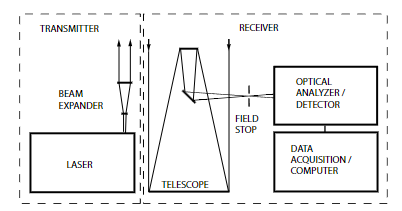
\includegraphics[bb=0in 0in 2.5in 2.5in, height=2.5in, width=2.5in]{figures/lidarSetup.png}
  \captionof{figure}{Principle setup of a LiDAR system (\Textcite{wandinger2005})}
  \label{fig:lidarSetup}
\end{minipage}

Multiple forms of LiDAR systems can be used for various applications. For example, \Textcite{conti2024} compared two applications of LiDAR sensors in the use of an Italian town hall building. The two sensor applications are terrestrial and mobile laser scanners (TLS and MLS respectively). A terrestrial laser scanner uses a LiDAR sensor mounted on a tripod and scans the area around it. Meanwhile, the MLS is a handheld LiDAR sensor that can be carried and transported with one hand. Figure 2 shows a MLS and TLS device.

\begin{minipage}{\linewidth}
  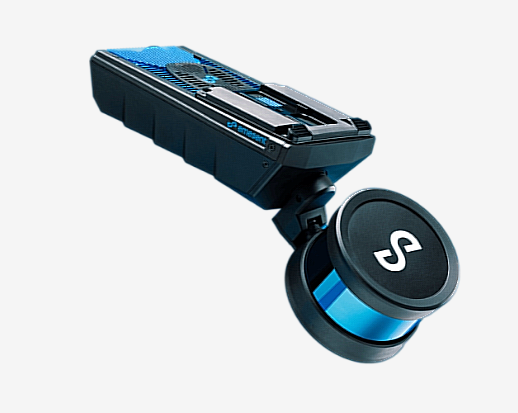
\includegraphics[height=\textheight/3,width=\textwidth/2]{figures/HoverMap.png}
  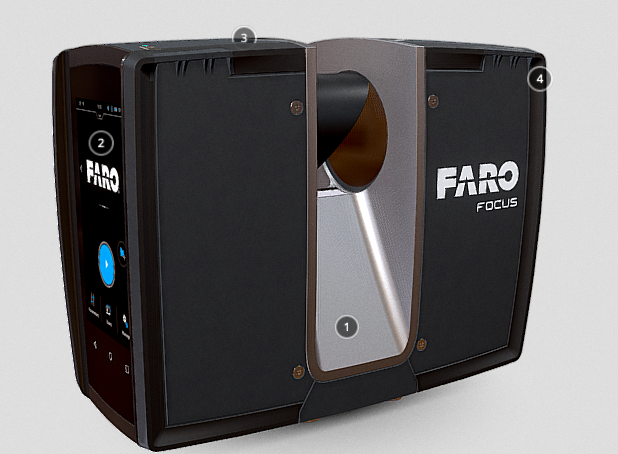
\includegraphics[height=\textheight/3,width=\textwidth/2]{figures/FaroFocus.png}
  \captionof{figure}{Hovermap Emesent MLS (left) (\Textcite{emesent}) and FAROFocus TLS (right) (\Textcite{FARO})}
  \label{fig:TLSandMLS}
\end{minipage}



\Textcite{conti2024} found that the MLS is able to create a streamlined and efficient workflow that is suitable for the documentation of heritage buildings. However, where a higher level of detail is required, the TLS would be more suitable. In this report, I aim to investigate the differences in the MLS and TLS through using the LiDAR systems shown in figure 2. Dense point clouds will be obtained for each system before being compared using the open source software CloudCompare. This software has been shown to be able to compare two different point clouds and investigate their respective quality (\Textcite{girardeau2016}). 

The overall procedure in investigating both LiDAR systems involves with firstly determining hardware settings and object to be scanned, followed by performing the scan to create a dense point cloud. The resulting point clouds will then be aligned and compared to each other qualitative and quantitatively. More details regarding the project procedure will be discussed in the methods section.



\section{Method}

\subsection{Point Cloud Registration}
\subsubsection{Manual Alignment}


\section{Results}
Table~\ref{tab:BasicTable} summarizes the data. \lipsum[1-3]
\vspace{20pt}

\begin{minipage}{\linewidth}
  \captionof{table}{Sample Basic Table}
  \label{tab:BasicTable}
  \begin{tabular}{@{}llr@{}}         \toprule
  \multicolumn{2}{c}{Item}        \\ \cmidrule(r){1-2}
  Animal    & Description & Price \\ \midrule
  Gnat      & per gram    & 13.65 \\
            & each        &  0.01 \\
  Gnu       & stuffed     & 92.50 \\
  Emu       & stuffed     & 33.33 \\
  Armadillo & frozen      &  8.99 \\ \bottomrule
  \end{tabular}
\end{minipage}

\vspace{20pt}

\lipsum[1]

Figure~\ref{fig:Figure1} shows this trend.

\vspace{20pt}
\begin{minipage}{\linewidth}
  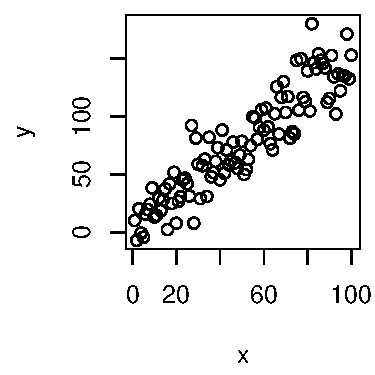
\includegraphics[bb=0in 0in 2.5in 2.5in, height=2.5in, width=2.5in]{figures/Figure1.pdf}
  \captionof{figure}{This is my first figure caption.}
  \label{fig:Figure1}
\end{minipage}

\section{Discussion}
\lipsum[17]

\lipsum[18]

\lipsum[19]

\printbibliography


\end{document}

%% 
%% Copyright (C) 2021 by Daniel A. Weiss <daniel.weiss.led at gmail.com>
%% 
%% This work may be distributed and/or modified under the
%% conditions of the LaTeX Project Public License (LPPL), either
%% version 1.3c of this license or (at your option) any later
%% version.  The latest version of this license is in the file:
%% 
%% http://www.latex-project.org/lppl.txt
%% 
%% Users may freely modify these files without permission, as long as the
%% copyright line and this statement are maintained intact.
%% 
%% This work is not endorsed by, affiliated with, or probably even known
%% by, the American Psychological Association.
%% 
%% 
%% This work is "maintained" (as per LPPL maintenance status) by
%% Daniel A. Weiss.
%% 
%% This work consists of the file  apa7.dtx
%% and the derived files           apa7.ins,
%%                                 apa7.cls,
%%                                 apa7.pdf,
%%                                 README,
%%                                 APA7american.txt,
%%                                 APA7british.txt,
%%                                 APA7dutch.txt,
%%                                 APA7english.txt,
%%                                 APA7french.txt,
%%                                 APA7german.txt,
%%                                 APA7ngerman.txt,
%%                                 APA7greek.txt,
%%                                 APA7czech.txt,
%%                                 APA7turkish.txt,
%%                                 APA7endfloat.cfg,
%%                                 Figure1.pdf,
%%                                 shortsample.tex,
%%                                 longsample.tex, and
%%                                 bibliography.bib.
%% 
%%
%% End of file `./samples/longsample.tex'.
